\documentclass[a4paper,12pt,twoside]{article}
\usepackage[utf8]{inputenc}
\usepackage{polski}
\usepackage{verbatim}
\usepackage{lmodern}
\usepackage{graphicx}
\usepackage{lastpage}
\usepackage{fancyhdr}

\pagestyle{fancy}
\renewcommand{\headrulewidth}{0pt}
\fancyhead{}
\cfoot{Strona\;\thepage\;z\;\pageref{LastPage}}

\title{Eskulap - Specyfikacja Implementacyjna}
\date{14 grudnia 2020}
\author{Piotr Nowak\\Hubert Piłka\\Dominik Wawrzyniuk}

\begin{document}
\maketitle
\thispagestyle{empty}
\newpage
\tableofcontents
\newpage
\section{Środowisko programistyczne}
\begin{description}
\item[\texttt {Język }] - Java
\item[\texttt {IDE }] - NetBeans, Eclipse
\item[\texttt {System }] - Windows
\end{description}
\section{Algorytm}
Algorytm będzie działał w następujący sposób:
\begin{center}
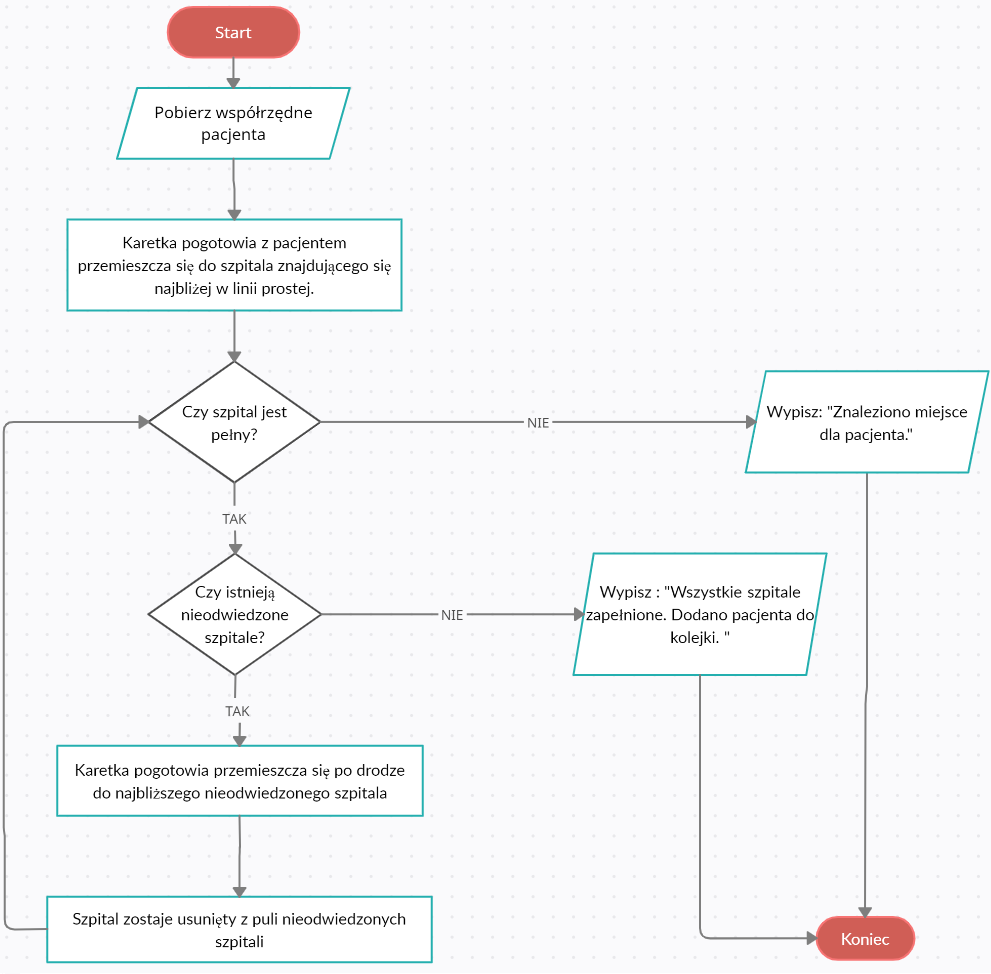
\includegraphics[scale=0.65]{schemat}
\end{center}
\section{Przewidywana struktura programu}
\begin{center}
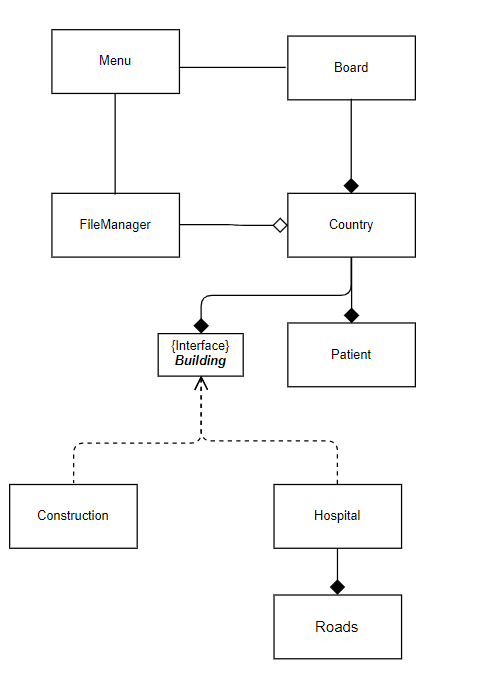
\includegraphics[scale=1.1]{struktura}
\end{center}
\newpage
\section{Ograniczenia danych wejściowych}
\subsection{Szpitale}
\begin{itemize}
\item id\\liczba całkowita z zakresu od 1 do 100
\item nazwa\\dane tekstowe o długości od 1 do 128 znaków
\item wsp. x\\liczba całkowita z zakresu od INT\_MIN do INT\_MAX
\item wsp. y\\liczba całkowita z zakresu od INT\_MIN do INT\_MAX
\item Liczba łóżek\\liczba całkowita z zakresu od 0 do INT\_MAX
\item Liczba wolnych łóżek\\liczba całkowita z zakresu od 0 do INT\_MAX
\end{itemize}
\subsection{Obiekty}
\begin{itemize}
\item id\\liczba całkowita z zakresu od 1 do 100
\item nazwa\\dane tekstowe o długości od 1 do 128 znaków
\item wsp. x\\liczba całkowita z zakresu od INT\_MIN do INT\_MAX
\item wsp. y\\liczba całkowita z zakresu od INT\_MIN do INT\_MAX
\end{itemize}
\newpage
\subsection{Drogi}
 Nie musi istnieć bezpośrednie połączenie między każdym szpitalem.\\Z każdego szpitala musi istnieć możliwość przemieszczenia się do każdego innego szpitala.
\begin{itemize}
\item id\\liczba całkowita z zakresu 1 - 4950
\\(w skrajnym przypadku, gdy istnieje bezpośrednie połączenie między każdym szpitalem ilość dróg
jest równa liczbie krawędzi w grafie pełnym $K_n$, gdzie n - ilość szpitali)\\dla n = 100
\\${\qquad\frac{n(n-1)}{2}} = 4950$
\item nazwa\\dane tekstowe o długości od 1 do 128 znaków
\item id\_szpitala\\liczba całkowita z zakresu od INT\_MIN do INT\_MAX
\item odległość\\liczba całkowita z zakresu od 0 do INT\_MAX
\end{itemize}
\subsection{Pacjenci}
\begin{itemize}
\item id\\liczba całkowita z zakresu 1 - 10 000
\item wsp. x\\liczba całkowita z zakresu od INT\_MIN do INT\_MAX
\item wsp. y\\liczba całkowita z zakresu od INT\_MIN do INT\_MAX
\end{itemize}
\section{Ograniczenia pozostałych danych}
\subsection{Skrzyżowania}
Na przecięciach dróg powstają skrzyżowania, których współrzędne zostają zaokrąglone w dół do liczb całkowitych.\\Odległości od skrzyżowań do aptek również zostają zaokrąglone w dół do liczb całkowitych.
\section{Testy}
\subsection{Forma testów}
Zostaną przeprowadzone testy jednostkowe za pomocą biblioteki JUnit.
\subsection{Przewidywane testy danych wejściowych}
\begin{enumerate}
	\item Brak nazwy pliku.
	\item Pusty plik wejściowy.
	\item Brakujące dane.
	\item Wartości spoza zakresu określonego w ograniczeniach danych wejściowych.
	\item Przerwy w sieci dróg.
\end{enumerate}
\subsection{Przewidywane testy poprawności algorytmu}
\begin{enumerate}
\item Więcej pacjentów niż miejsc w szpitalach.
\end{enumerate}
\end{document}